\documentclass[../main.tex]{subfiles}
\begin{document}
Greedy algorithm is a further optimization strategy on top of dynamic programming. It usually  constructs and tracks a single optimal solution to problem directly and incrementally; like the dynamic programming, it works with subproblems, and at each step it extends the last partial solution by evaluating all available candidates and then pick the best one at the moment without regard to other discarded solutions.  Greedy algorithm picks the best immediate output, but does not consider the big picture, hence it is considered greedy.

Because of the ``greediness'' of the greedy algorithms, whether the single one solution we derive is optimal or not is what for us to ponder and decide. The consciousness of its optimality is important: if we require an absolutely optimal solution, we have to prove its optimality with systematic induction methods, if we are aware that it wont lead to the optimal solution, but is close enough and a good approximation to the optimal solution that we seek but too expensive to achieve, we can still go for it. This chapter is a systematic study of the greedy algorithm, we focus on designing and proving methods that always try to achieve the optimal solution. 

Greedy algorithm is highly related to and relies on \textbf{math optimization}. It is ``easy'' if you can reason a solution and prove it easily with math, which comes ``natural''.  Greedy algorithm can be ``hard'' when we need to identify important and less obvious properties,  design a greedy approach, and prove its correctness with more systematic induction methods; it requires even more analysis effort than dynamic programming does. Because of the highly flexibility of the greedy algorithms, a lot algorithmic books do not even cover this topic. 
It is not frequently seen in real interviews, but we want to cover it because in the field of AI, the searching is approximate, greedy algorithm can be approximate too and efficient. Maybe it will inspire us in other fields. 


%%%%%%%%%%%%%%%%%%From dynamic programming to greedy algorithm%%%%%%%%%%%%%%%%%%%%%%%%%%%%
\section{Exploring}
\paragraph{Maximum Non-overlapping Intervals (L435)} Given a collection of intervals, find the minimum number of intervals you need to remove to make the rest of the intervals non-overlapping. Note: You may assume the interval’s end point is always bigger than its start point. Intervals like [1,2] and [2,3] have borders “touching” but they don’t overlap each other.
\begin{lstlisting}[numbers=none]
Example 1:

Input: [ [1,2], [2,3], [3,4], [1,3] ]
Output: 1
Explanation: [1,3] can be removed and the rest of intervals are non-overlapping.
\end{lstlisting}
\paragraph{Analysis} Naively, this is a combination problem that each interval can be taken or not taken, which has a total of $O(2^n)$ combinations. For each combination, we make sure its a feasible that none of the within items overlaps. The process of enumerating the combination has been well explained  in the chapter of search and combinatorics. As a routine for optimization problem, we use a sequence $X$ to represent if each item in the original array is chosen or not, $x_i\in \{0, 1\}$. Our objective is to optimize the value:
\begin{align}
    o = \max \sum_{i=0}^{n-1} x_i \\
    % \texttt{w.r.t} x_i\in \{0, 1\} \texttt{ and x_i does not overlap with each other}
\end{align}
However, if we sort the items by either start or end time, the checking of an item's compatibility to a combination will be only need to compare it with its last item

% Think further that in our resulting subsequence, if we sort them in order of their start time or finish time, we could have $s_i < f_i \leq s_{i+1} < f_{i+1}$. This would indicates that we sort our array of intervals in some order and simply the search space from a search tree to linear space. 
\subsubsection{Dynamic Programming}
\begin{figure}[H]
    \centering
    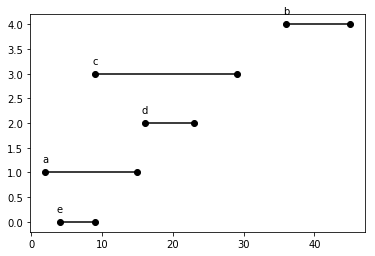
\includegraphics[width=0.49\columnwidth]{fig/greedy_schedule_all_intervals_sorting_finish.png}
    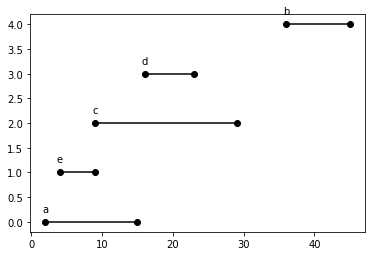
\includegraphics[width=0.49\columnwidth]{fig/greedy_schedule_all_intervals_sorting.png}
    \caption{All intervals sorted by start and end time.}
    \label{fig:greedy_intervals_sort_types}
\end{figure}
\paragraph{A-B: Convert to Longest Increasing Subsequence}   A feasible solution would be that $a_0, a_1, ..., a_k$, and $s(a_i)\leq f(a_i)\leq s(a_{i+1}) < f(a_{i+1})$. If we sort the intervals by either start or end time, our sorted intervals as shown in Fig.~\ref{fig:greedy_intervals_sort_types}. We can reduce our problem  into finding the length of longest subsequence $LS, i = [0, k-1]$ that does not overlap , which is equivalently defining  that $s[i+1]\geq f[i]$ in the resulting subsequence. This is similar enough to the concept of longest increasing subsequence, we can apply the dynamic programming to solve this problem with a time complexity of $O(n^2)$. 

For this problem, there can exist multiple optimal solutions and dynamic programming can tell us from the \texttt{LIS} array that which one has the maximum. Let's define a subproblem $d[i]$ as getting the maximum number of non-overlapping intervals for subarray $[a[0], a[1], ..., a[i-1]]$ with the maximum subsequence that includes $a[i-1]$. Then, our the recurrence relation is:
\begin{align}
    d[i]&=\max(d[j])+1, j \in [0, i-1], j <i, f(j) < s(i).
\end{align}
And the answer is $\max(d[i]), i \in[0, n-1]$.
\begin{lstlisting}[language=Python]
from typing import List 
def eraseOverlapIntervals(intervals: List[List[int]]) -> int:
    if not intervals:
        return 0
    intervals.sort(key=lambda x: x[0])
    n = len(intervals)
    LIS = [0]*(n+1) 
    for i in range(n): 
        max_before = 0
        for j in range(i, -1, -1): 
            if intervals[i][0] >= intervals[j][1]:
                max_before = max(max_before, LIS[j+1])
        LIS[i+1] = max(LIS[i], max_before+1)
    #print(LIS)
    return len(intervals)-max(LIS)
\end{lstlisting}

\paragraph{Simplified Dynamic Programming}
Let's approach the problem directly, define a subproblem $d[i]$ as the maximum number of non-overlapping intervals for subarray $a[0:i]$. 
With induction, assume we have solved all subproblems from $d[0]$ up till $d[i-1]$, meaning we have known the answer to all these subproblems.  Now we want to find the recurrence relation between subproblem $d[i]$ and its preceding subproblems. We have $a[i]$ at hand, what effect it can have? 

We can either increase its previous maximum value which is $d[i-1]$ by one, or else, the optimal solution remains unchanged. This makes the $d$ array   \textbf{non-decreasing} sequence. With this characteristic, we do not need to try out all preceding compatible intervals, but instead just its nearest preceding one--because it is at least the same as all preceding ones.  We define this preceding compatible interval of $a[i]$ with index $p[i]$, then our recurrence relation become 
\begin{equation}
    d[i] = max(d[i-1], d[p[i]]+1).
\end{equation}
And the final answer will be \texttt{dp[-1]}.
With the sorting, the part with the dynamic programming only takes $O(n)$, making the total time $O(n\log n)$ mainly caused by sorting. The Code only differs one line with the above approach:
\begin{lstlisting}[language=Python]
def eraseOverlapIntervals(intervals: List[List[int]]) -> int:
    if not intervals:
        return 0
    intervals.sort(key=lambda x: x[0])
    n = len(intervals)
    dp = [0]*(n+1) 

    for i in range(n): 
        max_before = 0
        for j in range(i, -1, -1): 
            if intervals[i][0] >= intervals[j][1]:
                max_before = max(max_before, dp[j+1])
                break
        dp[i+1] = max(dp[i], max_before+1)
    #print(LIS)
    return n-dp[-1]
\end{lstlisting}
\subsubsection{Greedy Algorithm} 
In the previous solution, the process looks like this: If it is sorted by end time, first we have $e, m = 1$, for $a$, it is not compatible with $e$, according to previous recurrence relation, $m=1$, with either $a$ or $e$ in the optimal solution. When we are processing $d$, its preceding compatible interval is $e$, making our maximum value $2$ for this subproblem. For $c$, the length of the optimal solution remains the same, but with additional optimal solution: $e, c$. 
However, if we go back, when we are processing $a$, is it necessary to keep $a$ and $e$ as the optimal solution. If we just get the maximum length of the optimal solution, we do not need to track all optimal solutions, but just one that is the most ``optimistic'', which will be $e$ in our case. Because choosing $e$ instead of $a$ leaves more space  and thus more likely to fit more intervals for the later subproblems. Similarly, for $c$, it is incompatible with $d$, then it is safe to throw it away, because it has the largest end time--the least optimistic, thus it is unnecessary to replace any previous interval in the optimal solution with it. This algorithm  takes this simplification even more aggressive and ``greedy'. Therefore, in the greedy algorithm, if we have multiple optimal solutions, usually it only cares about \textbf{one} that is the most promising and optimistic, and incrementally to build up on it. The code is given:
\begin{lstlisting}[language=Python]
def eraseOverlapIntervals(intervals: List[List[int]]) -> int:
    if not intervals:
        return 0
    min_rmv = 0
    intervals.sort(key = lambda x: x[1])
    last_end = -sys.maxsize
    for i in intervals:
        if i[0] >=  last_end: #non-overlap
          last_end = i[1]            
        else:
          min_rmv += 1
           
    return min_rmv
\end{lstlisting}
If we sort our problems by start time. We need to tweak the code a bit, that whenever one interval is incompatible with previous, we see if it has earlier end time that the previous one, if it is, then we replace it with this one, because it has later start time, and earlier end time, whatever the optimal that the previous interval is in, replacing it with the current one will not overlap and it will be more promising.
\begin{lstlisting}[language=Python]
for i in intervals:
    if i[0] < last_end: #overlap, delete this one, do not update the end
        if i[1] < last_end:
            last_end = i[1]
        min_rmv += 1
    else:
        last_end = i[1]
\end{lstlisting}
\subsubsection{Summary and Comparison}
We have seen that both dynamic programming and the greedy algorithms solves the problems \textbf{incrementally}--starting from small problems to larger problems. Dynamic programming plays safe by tracking the previous state, thus it does not matter how you sort these intervals; both by start time and end time work the same. However, in the greedy approach, it cares less about the previous states. 


For example, if our intervals are [[1, 11], [2, 12], [13, 14], [11, 22]], the dynamic programming will give us LIS=[0, 1, 1, 2, 2], which indicates there are two optimal solutions. While, in the greedy algorithm, we would find one that is [1, 11], [13, 14]. 
The resulting is, we might find a solution that is one of its multiple optimal solutions with the same length. In this process, we greatly increased our time efficiency, and simplified the algorithm design and coding. 

\paragraph{Questions to Ponder} 
\begin{itemize}
    \item Are you absolutely sure that is one of the optimal solutions? If it is optimal, how to prove it then?
    \item When can I use greedy algorithm over dynamic programming? 
\end{itemize}
% The first problem is challenging and it differs to different problems. There 

% To answer the second question first: We can't. The reason why greedy approach in the interval case is we have $s_i \leq f_i, f_i \leq f_{i+1}$. In the LIS, we have $s_i \leq f_i, s_{i+1}\geq f_i$. There is a \textbf{non-decreasing property}. This is very similar to our shortest-path graph algorithms. This is equivalently same as in an array [1, 2, 2, 3, 4, 4], to find the longest increasing subsequence and the greedy approach is to choose 1 first, and then 2. For the second 2, we compare it with previous 2, it is not larger, thus we skip it. With this greedy approach, we eventually get [1, 2, 3, 4] as the longest increasing subsequence. 

% For the third question, I find it is genuinely true that we need to have this non-decreasing property. We will see a lot in our real examples and they all point to this conclusion. 
\begin{bclogo}[couleur = blue!30, arrondi=0.1,logo=\bccrayon,ombre=true]{What if there each interval is weighted with a real value $w_i$, and the objective is to maximize a non-overlap set of interval's sum of weights? } {If the weight can be both negative and positive, we have to use the first dynamic programming method. If for every $w_i\geq 0$,  then previous suboptimal solution can still have a chance to lead to a global optimal solution if it happens to be compatible with following intervals with large weight, we can apply the second dynamic programming method.  }
\end{bclogo} 

%%%%%%%%%%%%%%%%%%%%%%%%%%%%%%%%%%%%%%%
\section{Introduction to Greedy Algorithm} 
\subsubsection{What is Greedy Algorithm?} We say that dynamic programming tracks best solution to all subproblems (in the above example, it is the \texttt{d} array) and incrementally build up solutions to subproblems using their subproblems  (in our example, we use all of its subproblems \texttt{for j in range(i)} to build up solution to subproblem \texttt{d[i]}.

% While, it is hard to give precise definition of greedy algorithms. In \textit{introduction to algorithms}, it defines two properties to greedy algorithms but I often found it is confusing to match the implementation to the definition:


% \paragraph{check later}
% While, greedy algorithm does not track or solve all subproblems. It approaches the problem from a different way! If we make a greedy choice, we have only one remaining subprpblem to solve: for example, at first, we greedily choose [1,11], leaving us with one subproblem [2, 12], [13, 14], [11, 22]. Then, we check [2, 12], which is not compatible to its solution [1, 11], we skip, and leaving our subproblem as  [13, 14], [11, 22]. Then we check [13, 14], add into our partial optimal solution, and we have a subproblem even smaller to solve later. As the process of greedy algorithm, we are always downsizing our remaining subproblem. In dynamic programming solution, each subproblem will have an answer in \texttt{LIS}. However, for the greedy approach, we do not know and in instead, it directly select an item as part of our optional solution at each step. 
Greedy algorithm follows the same trend in the sense of solving overlapping subproblems where  optimal substructure property shows. But it only maintain  \textbf{one optimal solution} for each of the subproblem--the most promising one. For example, for [[1, 11]], the optimal solution is [1, 11], for [1, 11], [2, 12], the optimal solution is still [1, 11], even though [2, 12] is another optimal solution for this subproblem.  For [1, 11], [2, 12], [13, 14], [11, 22], greedy approach gives us [1,11],[13, 14] as our optimal solution, while in dynamic programming, we can still find another optimal solution: [1, 11], [11, 22]. 
\paragraph{Three Properties} We define three properties for greedy algorithm:
\begin{itemize}
    \item Overlapping Subproblems and Optimal substructure property: These two properties defined exactly the same as in dynamic programming. If an optimal solution to the problem contains within it optimal solutions to its subproblem, this is said to be optimal substructure. In our example, [1, 11], [2, 12], [13, 14], the optimal solution [1, 11], [13, 14] contains optimal solution [1, 11] that is to its subproblem [1, 11], [2, 12]. 
    \item Greedy-choice property: This is the only additional property that greedy algorithm holds compared with dynamic programming. We can assemble a globally optimal solution by making a locally optimal (greedy) choice. 
    
    For example, given an array [2, 1, 3, 7, 5, 6], which has as [1, 3, 5, 6], [2, 3, 5, 6] as the longest increasing subsequence. We define the LIS as the longest increasing subsequence that ends at a[i-1] for array $a[0:i]$. The process of constructing it with dynamic programming shows as follows:
    \begin{lstlisting}
    subproblems
    [2], LIS = [2]
    [2, 1], LIS = [1]
    [2, 1, 3], LIS= [1, 3], [2, 3]
    [2, 1, 3, 7], LIS = [1, 3, 7], [2, 3, 7]
    [2, 1, 3, 7, 5], LIS = [1, 3, 5], [2, 3, 5]
    [2, 1, 3, 7, 5, 6], LIS = [1, 3, 5, 6], [2, 3, 5, 6]
    \end{lstlisting}
    We clearly see that to get the best solution, we have to rely on the optimal solution of all preceding subproblems. If we insist on applying greedy algorithm, this is how to process looks like:
      \begin{lstlisting}
    subproblems
    [2], LIS = [2]
    [2, 1], LIS = [2], only compare [2] and 1
    [2, 1, 3], LIS= [2, 3]
    [2, 1, 3, 7], LIS = [2, 3, 7]
    [2, 1, 3, 7, 5], LIS = [2, 3, 7]
    [2, 1, 3, 7, 5, 6], LIS = [2, 3, 7]
    \end{lstlisting}
    LIS = [2, 3, 7] is locally optimal but not part of the global optimal solutions which are [1, 3, 5, 6] and [2, 3, 5, 6]. In our non-overlapping interval problem, if one interval is optimal in the local subproblem, it will sure be part of the optimal solution to the final problem (globally). 
    
    % While in greedy algorithm, because of the special ordering in our optimal solution $s_i \leq f_i, f_i \leq f_{i+1}$, and our ordering of our data decides the optimal solution only relies on one optimal solution of the previous subproblem. This will only work  if the data is ordered in some way. 
    
 
\end{itemize}
To summarize, greedy algorithms simply works on incrementally build up one optimal solution. For this single optimal solution to be globally optimal, each partial optimal solution has to exactly match some prefix of the optimal solution. Both proving the correctness and design of greedy algorithm thus has to be done by induction and that at each stage, greedy algorithm is making the best choices.  

To  correctly design a greedy algorithm, it has to make a locally optimal choice according to some rules or orderings.  In the above example, we know the optional solution has the property that $s_i \leq f_i, f_i \leq f_{i+1}$.     By sorting the intervals with increasing order of the finish time. The greedy approach choose the interval with the earliest finish time, and it says, this belongs to my optimal solution. And it just need to go through all the candidates in the order of finishing time and see if it is compatible with the last item, and we would build up a feasible and optimal solution. It orders its subproblems to make sure each partial optimal solution will be ``prefix'' or part of the global optimal solution. 
\subsubsection{Practical Guideline}
It is clear to us like in dynamic programming, greedy algorithms are for solving optimization problems, and it subjects to a set of constraints. For example:
\begin{itemize}
    \item Maximize the number of events you can attend, but do not attend any overlapping events.
    \item Minimize the number of jumps
    \item Minimize the cost of all edges chosen, but do not disconnect the graph.
\end{itemize}

Do not worry about the definition of greedy algorithm; it is hard and often confusing, because it is a natural and highly dependable on the problem context. However, to come up with a rule that. 

I suggest we start with dynamic programming, it is more systemized, easier to prove the correctness, and it guides us to walk through to the greedy algorithm which is more efficient just as the process shown in the example. 
\paragraph{Ordering, Monotone Property} These constraints bring sense of ordering in our optimal solution, and this is when greedy algorithm applies. Therefore, we say:``beneath every greedy algorithm, there is almost always a more cumbersome dynamic programming solutions''. But, not every dynamic programming we can find a more efficiency greedy algorithm, because to make greedy algorithm work, there needs to have some ordering in the optimal solution that makes the locally optimization applicably and globally optimal. We shall see this in our examples! In the activity scheduling, it is that $d[i]$ is non-decreasing as shown in its dynamic programming solution. Because of this property, a glo therefore, and in the dijkstra's algorithm, it is that $w(s, u) < w(s, v) = w(s, u) + w(u, v)$.  in the shortest path. Once this monotone property breaks as in a graph with negative weights, greedy algorithm won't apply and we have to retreat to dynamic programming. 

\subsubsection{Pros and Cons}
As we see, greedy algorithm has the following pros:
\begin{itemize}
    \item     Simplicity: Greedy algorithms are often easier to describe and code up than other algorithms.
    \item Efficiency: Greedy algorithms can often be implemented more efficiently than other algorithms.
\end{itemize}
However, 
\begin{itemize}
    \item Hard to get it right: Once you have found the right greedy approach, designing greedy algorithms can be easy. However, finding the right rule can be hard.
    \item Hard to verify/prove: Showing a greedy algorithm is correct often requires a nuanced argument.
\end{itemize}
%%%%%%%%%%%%%%%%%%%%%Prove Greedy Algorithm%%%%%%%%%%%%%%%%%%%%%%%%%
\section{*Proof}
The main challenging in greedy algorithms is to prove its correctness, which is important in theoretical study. However, in real coding practice, we can leverage the dynamic programming solution to compare with and scrutinize different kinds of examples to make sure the greedy algorithm and the dynamic programming are having the same results. Still, let us just learn this proof techniques as mastering another powerful tool. 

\subsection{Introduction}
First, we introduce generally two techniques/arguments to prove the correctness of a greedy algorithm in a step-by-step fashion using the mathematical induction, they are: \textbf{Greedy Stays Ahead} and \textbf{Exchange Arguments}.
\subsubsection{Greedy stays ahead}
This simple style of proof works by showing that, according to some measures, the optimal solution built by the greedy algorithm is always at least or better than the optimal solution during each iteration of the algorithm. Once we have established this argument, we can show that the greedy solution must be optimal. Typically there are four steps:
    \begin{enumerate}
        \item Define the solution: Define our greedy solution as $G$ and we compare it against some optimal solution $O^{*}$.
        \item Define the measurement: Your goal is to find a series of measurements you can make of your solution and the optimal solution.  Define some series of measures $m_1(X), m_2(X), ..., m_n(X)$ such that $m_1(X^{*}), m_2(X^{*}), ..., m_k(X^{*})$ is also defined for some choices of m and n.Note that there might be a different number of measures for X and X*, since you can't assume at this point that X is optimal
        \item Prove Greedy Stays Ahead: Prove that $m_i(X)\geq m_i(X^{*})$ or that  $m_i(X)\leq m_i(X^{*})$, whichever is appropriate, for all reasonable values of $i$. This argument is usually done inductively.
        \item Prove Optimality.  Using the fact that greedy stays ahead, prove that the greedy algorithm must produce an optimal solution.  This argument is often done by contradiction by assuming the greedy solution isn't optimal and using the fact that greedy stays ahead to de-rive a contradiction.
    \end{enumerate}
    The main challenge with this style of argument is finding the right measurements to make. 
\subsubsection{Exchange Arguments} It proves that the greedy solution is optimal by showing that we can iteratively \textbf{transform} any optimal solution into the greedy solution produced by greedy algorithm without worsening the cost of the optimal solution. This transformality matches the word ``exchange''. Exchange arguments are a more versatile technique compared with greedy stays ahead. 
It can be generalized into three steps:
\begin{enumerate}
    \item Define the solution: Define our greedy solution as $G=\{g_1, ..., g_k\}$ and we compare it against some optimal solution $O=\{o_1, ..., o_m\}$.
    \item Compare solutions: Assume the optimal solution is not the same as the greedy solution; show that if $m(G)\neq m(O)$, then $G$ and $O$ must  differ in some way. How it differs depend on the measurement and the problem context. 
    \begin{enumerate}
        \item If it is a combination and a length problem, then $m(G)=k$, and $m(O)=m$, we need to prove $k=m$.
        \item If it is a combination and with objective as a value, we assume $o_1$ and $g_1$ differs and all others are identical. Then, we swap $o_1$ with $g_1$. 
        \item If it is a permutation with objective function, we assume there are two consecutive items in $O$ that is in a different order than they are in $G$ (i.e. there is inversion)
    \end{enumerate}
    \item Exchange Arguments: Show how to transform $O$ by exchanging some piece of $O$ for some piece of $G$. Then, we prove that by doing so, we did not increase/decrease the cost of $O$ as we transform $O$ to $G$ with more iterations, proving that greedy is just as good as any optimal solution and hence is optimal. 
    % \item Iterate: Argue that we have decreased the number of difference between $G$ and $O$ by performing exchange, and with the iteration we can turn $O$ into $G$ without impacting the quality of the solution. Therefore, $G$ must be optimal. 
\end{enumerate}

\subsubsection{Guideline}
We will simply go through the list and, but the point is it is we should use the proof methods as a way to design the greedy algorithm on top of the dynamic programming. 

\subsection{Greedy Stays Ahead}
\paragraph{Maximum Non-overlapping Intervals Proofs} Let's use $G, O$ for our greedy and optimal solution respectively. $G$ consists of $\{G_1, G_2, ..., G_k\}$ in the order they each item is added into the $G$. Similiarly, $O_1, O_2, ..., O_m$ is  one of the optimal sets. 
\begin{theorem}
$G$ is a compatible set of intervals.
\end{theorem}
$G$ is trivially feasible because in our design we discard any interval that overlaps with our previous greedy choice. Now, all it matters is to prove its optimality. 

We know that there might exist multiple optimal solutions for a problem, just as shown in our example. In this particular problem, we do not intend to prove that $G=O$, because it might not; we prove that $G$ and $O$ has the same length instead $|G|=|O|$. We will apply ``greedy stays ahead'' principle along with mathematical induction. We first assume that the intervals in $O$ is ordered by the same rule applied on $G$--$f(O_i)<f(O_j)$, if $i<j$. In this case, we use the finishing time $f$ of each interval to measure. To prove $|G|=|O|$, we need to prove Greedy stays ahead and the optimality.
\begin{theorem}\label{greedy_stays_ahead}
$f(G_i)\leq f(O_i), i \in [1, k]$, 
\end{theorem}
For $i=1$, the statement is true: our algorithm starts by choosing interval with minimum finish time. We further assume the statement is true for $n-1$ as our induction hypothesis. \ref{greedy_stays_ahead} will be proved if we can prove that $f(G_n) \leq f(O_n)$. 

$f(G_{n-1})\leq f(O_{n-1}) \leq s(O_n)$ tells us: right after the selection of $G_{n-1}$, $O_n$ together with others remains in the available set for the selection at step $n$--$f(O_{n-1}) \leq s(O_n)$ is always true because $O$ is a compatible set, and naturally, $f(O_n)>s(O_n)\geq f(O_{n-1})$. The greedy algorithm selects the available interval with smallest finish time, which guarantee that $f(G_n)\leq f(O_n)$. Now, we have formally proved our sense of ``greedy stays ahead'' or rather ``greedy never fall behind'' using induction. 
\begin{theorem}\label{prove_optimality}
$G$ is optimal: $|G|=|O|$. 
\end{theorem}
We apply contradiction: if $G$ is not optimal, then we must have $m>k$. Similarily, after step $k$, we have $f(G_{k})\leq f(O_{k}) \leq s(O_{k+1})$, and $O_{k+1}$ must be remaining in the available set for greedy algorithm to choose. Because greedy algorithm only stops when the remaining set is empty--a contradiction. So far, we successfully applied the ``greedy stays ahead'' method to prove the correctness in the example of maximum non-overlapping intervals. 

\subsection{Exchange Arguments}


\paragraph{Scheduling to minimize lateness: } Instead of having a fixed start and end time for each interval, we relax the start time. Therefore, we represent the interval with $[t_i, d_i]$, where $t_i$ is the contiguous time interval and $d_i$ is the deadline. There are many objective functions we might want to optimize. Here, we assume we only have one resource, what is the maximum number of meetings that we can schedule into a single conference room and none of them is late or we allow some meetings to run late, but define lateness $l_i$ as:
\begin{equation}
    l[i] =
    f[i] - d[i]
\end{equation}
Say, our object is to minimize the total lateness scheduling all meetings in one conference room, find the optimal solution: 
\begin{align}
    O&=\min \sum_{i=0}^{n-1} l_i\\
    &=\min \sum_{i=0}^{n-1} f[i] - d[i]
\end{align}
\begin{lstlisting}[numbers=none]
For example, we have nums = [[4, 6], [2, 6], [5, 5]]
The optimal solution is [2, 6],  [4, 6], [5, 5] with total lateness  (2-6)+(2+4-6)+(2+4+5)-5 = -4+0+6 = 2
Example 2:
nums = [[2,15],[36,45],[9,29],[16,23],[7, 9], [4,9], [5, 9]]
ans = 47
\end{lstlisting}
\paragraph{Analysis} First, let us assume all intervals have distinct deadline. A naive solution is to try all permutation of $n$ intervals and find the one with the minimum lateness. But what if we start from random order, we compute its lateness and each time we exchange two adjacent items and see if this change will decrease the total lateness or not. 
\begin{lstlisting}
______a_i____a_j
\end{lstlisting}
Therefore, 
Say our items are $a_i$ and $a_{j}$. There are four cases according to $d_i, d_{j}, t_i, t_{j}$. At first, with lateness $s + t_i -d_i$, and $s+t_i+t_j-d_j$. After the exchange, we have $s+t_j - d_j$ and $s+t_j+t_i - d_i$. $i$ will definitely be more late, $j$ however will be less late. Let us compare the additional lateness of $i$ with the decreased lateness of $j$:
    \begin{align}
        s+t_j+t_i - d_i - (s+t_i-d_i) \xrightarrow{} s+t_i+t_j-d_j - (s+t_j-d_j) \\
        t_j \xrightarrow{} t_i
    \end{align}
Therefore, we have to exchange $i,j$ if $t_j < t_i$. Thus, ordering the list with increasing order of duration time of each meeting will have the best objective. Our Python code is:
\begin{lstlisting}[language=Python]
def lateness(intervals):
  intervals = sorted(intervals, key=lambda x: (x[0]))
  f = 0
  ans = 0
  for i, (t, d) in enumerate(intervals):
    f += t
    ans = ans + f-d 
  return ans
\end{lstlisting}
\paragraph{Modification} However, if we modify our definition of lateness as:
\begin{equation}
    l[i] = \begin{cases} 0, & \text{if } f[i] \leq d[i], \\
    f[i] - d[i], \text{otherwise}.
    \end{cases}
\end{equation}
Which is to say we do not reward for intervals that are not late with negative values. Things get more complex. 

\begin{enumerate}
    \item If none of them is late, then exchange or not to change will not make any difference to the total lateness. 
\begin{lstlisting}
______a_i____a_j__d_i__d_j
\end{lstlisting}
\item If both is late, then exchange the items if $t_j <  t_i$.
\item If $i$ is late, and $j$ is not late, then no matter about their $t$, exchange them will only be even later. 
\item If $i$ is not late, and $j$ is late. Exchange them will totally depends
\end{enumerate}
Therefore, if we change the definition of lateness, greedy solution is no longer available for us, not even dynamic programming. But the greedy approach that first sorts the intervals by the duration time will get us a good start, then we can track the smallest lateness with backtracking and search prune by its minimum lateness found so far. 
\begin{lstlisting}[language=Python]
def lateness(intervals, f, l, globalmin, globalans, ans, used):
  if len(ans) == len(intervals):
    if l < globalmin[0]:
      globalmin[0] = l
      globalans[0] = ans[::]
    return 
  for i, (t, d) in enumerate(intervals):
    if used[i]:
      continue
    used[i] = True
    f += t
    if f-d >= 0:
      l+= (f-d)
    if l < globalmin[0]:
      ans.append(i)
      lateness(intervals, f, l, globalmin,globalans, ans, used )
      ans.pop()
    if f-d >=0:
      l -= (f-d)
    f -= t
    used[i] = False
  return 
\end{lstlisting}
We call this function with code:
\begin{lstlisting}[language=Python]
intervals = sorted(intervals, key=lambda x: (x[0]))
globalmin, globalans = [float('inf')], [[]]
ans = []
used = [False]*len(intervals)
lateness(intervals, 0, 0, globalmin, globalans, ans,  used)
print(globalmin, globalans[0])
for i in globalans[0]:
  print(intervals[i], end= ' ')
\end{lstlisting}
We will get the following output:
\begin{lstlisting}[numbers=none]
63 [1, 2, 0, 3, 4, 5, 6]
[4, 9] [5, 9] [2, 15] [7, 9] [9, 29] [16, 23] [36, 45] 
\end{lstlisting}
We can see that no particular rule--not sorting by $d$, not by $t$, and not by $d-t$ which is called \textbf{slack time}--we can find that to solve it in greedy polynomial time. However, can we use dynamic programming? 
\paragraph{Dynamic Programming} We can first do a simple experiment: we take out $[2, 15]$ from our \texttt{intervals}, the resulting optimal solution keeps the same order as [4, 9] [5, 9] [7, 9] [9, 29] [16, 23] [36, 45], which is a very good indicator that dynamic programming might apply. We can keep taking out and the optimal solution is still simply the same order, this indicates the optimal substructure. 

Let us assume we find the best order $O$ for subarray $intervals[0:i]$, now we have to prove that the best solution for subarray $intervals[0:i+1]$ can be obtained by inserting \texttt{interval[i]} into $O$. Assume the position we insert is at $j$, so $O[0:j]$ will not be affected at all, we care about $O[j:i]$. First, we have to prove that no matter where to add insert \texttt{interval[i]}, the ordering of $O$ needs to keep unchanged for it to have optimal solution. If insert position is at the end of $O$, the ordering do not need to change. For the other positions, however, it is really difficult to prove without enough math knowledge and optimization. 

Let us assume the start time is $s$ for $j, j+1$, we know:
\begin{align}
    l(s+t_j-d_j)+l(s+t_j+t_{j+1}-d_{j+1}) \leq l(s+t_{j+1}-d_{j+1})+l(s+t_j+t_{j+1}-d_{j})
\end{align}
Because $l(c)\in[0, c]$, prove that 
\begin{align}
    l(s+t_j+t_i-d_j)+l(s+t_j+t_i+t_{j+1}-d_{j+1} )\leq l(s+t_{j+1}+t_i-d_{j+1})+l(s+t_j+t_i+t_{j+1}-d_{j})
\end{align}

We can not prove it, and we use this method to try out, but it gives us wrong answer, so far, all our attempt to use greedy algorithm failed miserably. 


When there is a tie at the deadline, if we schedule the one that takes the most time first, we end up with higher lateness. For example, if our solution is [5, 5], [4, 6], [2, 6], the lateness is 5+4-6 + (9+2-6) = 3+5 =8 instead of 6. 

\begin{bclogo}[couleur = blue!30, arrondi=0.1,logo=\bccrayon,ombre=true]{What if each interval, if we are allowing multiple resources, what is the least number of conference rooms we need to schedule all meeting. } 
\end{bclogo}

\begin{bclogo}[couleur = blue!30, arrondi=0.1,logo=\bccrayon,ombre=true]{630. Course Schedule III, find the maximum number of non-overlapping meetings can be scheduled within one resource. } 
\end{bclogo}

\paragraph{Prove the Kruskal's Algorithm} Let the optimal minimum spanning tree be $O = (V, E^{*})$, and the one generated by greedy approach be $G=(V, E)$. $|E^{*}|=|E|$ because both is a tree and the number of edges always equal to $|V|-1$. Assume there is one edge $e\in E^{*}, e\not \in E$, this means that there is another edge $f \in E$ that differs from $e$. Other than these two edges, all the other edges are the same.  For example, in the graph we say $e=(1,5)$. With the constraint that there is only edge differs, $f$ has to be one edge out of $(2, 3), (3, 5)$; adding $e$ to $T$ forms a cycle, so in $T^{*}$, it can not have edges $(2, 3), (3, 5)$ at the same time, thus one referred as $f$ has to be removed in the $T^{*}$.  It is always true that $cost(e)\geq cost(f)$, because otherwise the greedy approach would have chosen $e$ instead of $f$.

For the optimal approach, if we replace $e$ with $f$, then we have $cost(T) =cost(T^{*}-e+f) \leq cost(T^{*})$. This means, with this swap of $e$ and $f$ between $G$ and $O$, the cost of the greedy approach is still at most the same as the optimal cost, transforming the optimal solution to greedy solution will not worsen the optimal solution. 

\section{Design Greedy Algorithm}
We have seen greedy algorithm design, definition, and different examples of greedy approaches and its proof. One obvious sign that states greedy approach might apply is, ``sorting will not incur the correctness of the optimal solution but rather greatly simplify the design complexity’’. Generally, people design a greedy algorithm by trying out rules with objection and hopefully find one good enough and then prove its correctness. This approach is simple but fuzzy. Thus, we prefer a more systemized design approach:
\begin{enumerate}
    \item Search: Analyze the problem with search and combination--no implementation is needed, to know our atomic search complexity. 
\item Dynamic Programming: Design dynamic programming approach first by defining state and constructing a recurrence relation repeatedly until we find one that works well.  This step brings us closer to the greedy approach: it gives us definition of state, recurrence relation and a polynomial time complexity.
\item Greedy: then further to see if the greedy choice property holds--between a subproblem $p_i$ and its succeeding subproblem $p_{i+1}$, if the optimal solution within $p\_i$ is also part of the optimal solution within $p\_{i+1}$ or we can simply construct an optimal solution from previous optimal solutions without checking multiple subproblems. If it holds, great, the previous dynamic programming becomes an overkill, and we further improve our approach by simplifying the recurrence relation with ``rules’’, which saves us time and/or space. To derive a good ``rule’’, we have to study and understand a bunch of ``facts’’, thus strengthen our choice with: Does the greedy optimal solution always stay ahead and be the most promising optimal solution at each step? If not, try exchanging some items within the previous optimal solution and see if it improves the situation and keeps us staying ahead. 
 \end{enumerate}
We will solve the following classical problems with this

%%%%%%%%%%%%%%%%%%Classical problems%%%%%%%%%%%%%%%
\section{Classical Problems}
List classical problems
\subsection{Scheduling}
We have seen two scheduling problems, it is a time-based problem which naturally follows has a leftmost to rightmost order along the timeline. And it is about scheduling tasks/meetings to allowed resources. We need to pay attention to the following contexts:
\begin{itemize}
    \item Do we have to assign all intervals or just select a maximum set from all? This relates to the number of resources that are available.  
    \item What are the conditions? Is both start and end time fixed, or they are highly flexible and are bounded by earliest possible start time and latest end time?
\end{itemize}
The core principle is to answer these questions:
\begin{itemize}
    \item Start and end time: 
    \begin{itemize}
        \item Is both fixed? Yes, then we are simply giving these intervals as a state, no change at all, and the ordering of the start and end time is exactly the same. If the question is only given one resource and we need to get the maximum non-overlapping intervals, easy piece of cake, we follows the order, and check if it is compatible with one previous intervals. If it asks about the minimum resources needed, that is the depth of the set, that is the property, we have discussed how assigning a meeting room to a preceding free meeting room does not affect the number of free rooms for the next. 
        \item If it is not fixed, we are given either $t_i$ and $d_i$ for each interval--we can start at any time $s_i$, finish at $s_i+t_i$, but we do have a deadline $d_i$ that better to be met--or we are given $b_i, t_i, d_i$--we can start at any $s_i$, but it would better be $s_i\geq b_i$, and end at $s_i+t_i\leq d_i$. (The second is not sure). The fundamental rule is: \textbf{Earliest Deadline First}. We have proved that if there is an inversion, swapping them will only result better objective value. This usually points out that the optimal solution shall have no inversion and no idle time on the resource. Whenever we met a tie at the deadlines, no matter what order of these intervals with equal deadline, the total lateness is usually the same, which can be proved with inversion. 
    \end{itemize}
\end{itemize}
\paragraph{Scheduling all Intervals(L253. Meeting Rooms II)} In our previous scheduling problem, there is only a single resource to fit in non-overlapping intervals. Scheduling all intervals on the other hand requires us to schedule all the intervals with as few resources as possible. This problem is also known as \textbf{interval partitioning problem} or \textbf{interval coloring problem} because our goal is to partition all intervals across multiple resources, and it is like each resource to be assigned a color.

Given an array of meeting time intervals consisting of start and end times $[[s_1,e_1],[s_2,e_2],...] (s_i < e_i)$, find the minimum number of conference rooms required and assign a label for each interval. 
\begin{lstlisting}[numbers=none]
Example 1:
Input: [[2,15, 'a'],[36,45, 'b'],[9,29, 'c'],[16,23, 'd'],[4,9, 'e']] 
Output: 2
\end{lstlisting}
\begin{figure}[H]
    \centering
    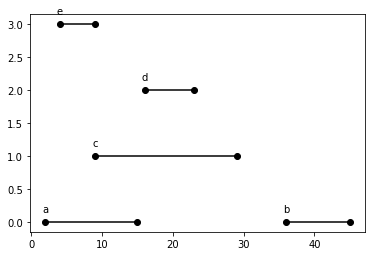
\includegraphics[width=0.7\columnwidth]{fig/greedy_schedule_all_intervals_1.png}
    \caption{All intervals}
    \label{fig:greedy_intervals}
\end{figure}
\paragraph{Analysis} The example is plotted in Fig.~\ref{fig:greedy_intervals}. A universal solution is to treat each interval as a vertex, if two intervals overlap, connect them with an edge, thus forming a graph. Now, the problem is reduced to a graph coloring, however, it might be to complicating things. 

\subsubsection{Find Minimum Number of Conference Rooms}
First, let us solve the first problem: What is the minimum number of conference rooms required? By observation and intuition, if at the same time point, there are a number of overlapping intervals, we have to assign each of these intervals a different resources. Now, we define the depth $d$ as the maximum number of overlapping intervals at any single point on the time-line, we claim: 
\begin{theorem}
In the interval partitioning problem, the number of resources needed is at least the depth $d$ of the set of intervals.
\end{theorem}
Before we head off to the proof, let's discuss how to find the depth. According to the definition, if we are lucky that the time given is in the form of integer, then, the most straightforward way is to use the \textbf{sweep line} method, with a \texttt{counter} to track the number of intervals at each integer time moment. We use a vertical line to sweep from the leftmost to the right most intervals: this exactly follows a natural order, that when the earliest meeting starts, we have to assign a room to it no matter what (start has +1), and when can  reuse a meeting room assigned before only if there is one that is freed (end has -1 as value). The sweep line method  We need to watch out for the edge case, when two intervals where the finish time of one and the start time of the other overlaps, such as $[4, 9], [9, 29]$, this is not counted as two. Therefore we make sure to exclude the finish time when scanning, in range $[s, e)$. 
\begin{figure}[H]
    \centering
    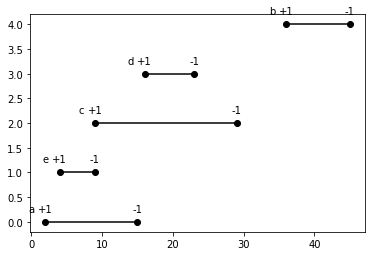
\includegraphics[width=0.7\columnwidth]{fig/greedy_schedule_all_intervals__sort_count.png}
    \caption{All intervals sorted by start and end time.}
    \label{fig:greedy_intervals_sort_count}
\end{figure}
However, this process can be simplified. When we are scanning, we will notice that the count will only change when encountering start or finish time point. First, at the start time of $a$, we have to assign one room, then at the start time of e, we have to assign a second room, and at the end of $e$, we free the room, and at the start time of $c$, it reuses the second room right away. Then in the line, at the end of $a$, it releases room 1, so $d$ starts reusing the first room right away. We can simply assign 1 to the start time, -1 to the finish time, and put all of these points into a list, sort them by time first. Because to handle the edge case--a tie in the previous sort where the start and end time is the same, the second degree sorting is used to put -1 in front of 1 to avoid overcounting the rooms. This process is shown in Fig.~\ref{fig:greedy_intervals_sort_count}.
\begin{lstlisting}[language=Python]
def minMeetingRooms(intervals):
    if not intervals:
        return 0
    points = []
    for s, e in intervals:
        points.append((s, +1))
        points.append((e, -1))
    points = sorted(points, key=lambda x: (x[0], x[1]))
    ans = 0
    total = 0
    for _, flag in points:
        total += flag
        ans = max(ans, total)
    return ans
\end{lstlisting}
\subsubsection{Label Assignment}
We can modify the previous code to incorporate label assignment.  We separate the start and end time in two independent lists because only when we meet a start time, we assign a room, and sort both of them. 
\begin{lstlisting}[numbers=none]
2(0) 4(4) 9(2) 16(3) 36(1)
9(4) 15(0) 23(3) 29(2) 45(1)
\end{lstlisting}
We put two pointers, $sp, ep$ at the start of the start time list and end time list respectively. We need zero room at first. And for start pointer at $2$, we assign room one to interval 0 because $2<9$, no room is freed to reuse. Then $sp$ moves to 4. $4<9$, no room is freed, assign room 2 to interval 4. $sp$ at 9, $9\geq9$, meaning we can reuse the room belonged to interval 4, thus assign room 2 to interval 2. Now, move both $sp$ and $ep$, we are comparing $16>15$, meaning interval 3 can reuse the room belonged to interval 0, we assign room 1 to interval 3. Next, we compare $36 > 23$, interval 1 takes the room number 1 from interval 3. Since one of the pointer reached to the end of the list, process ends.  
\begin{lstlisting}[language=Python]
def minMeetingRooms(intervals):
    starts, ends = [], []
    for i, (s, e) in enumerate(intervals):
        starts.append((s, i))
        ends.append((e, i))
    starts.sort(key=lambda x: x[0])
    ends.sort(key=lambda x: x[0])
    n = len(intervals)
    rooms = [0] * n
    sp, ep = 0, 0
    label = 0
    while sp < n:
        index = starts[sp][1]
        # Assign a new room
        if starts[sp][0] < ends[ep][0]:
            rooms[index] = label
            label += 1
        else: #Reuse a room
            room_of_end = rooms[ends[ep][1]]
            rooms[index] = room_of_end
            ep += 1
        sp += 1
    print(rooms)
    return label
\end{lstlisting}

The above method is natural but indeed greedy! We sort the intervals by start time, the worst case we assign each meeting a different room. However, the number of room can be reduced if we can reuse any previous assigned meeting rooms that is free at the moment.  \textbf{The depth is controlled by the time line}.  For example, for interval $c$, if both $a$ and $e$ is free at that moment, does it matter which meeting room to put of c in? Nope. Because no matter which room it is in, the interval d will overlap with this interval, thus can not use its meeting room, but still there is the one left from either a or e. This is what this problem is essentially different from the maximum non-overlapping problems. The greedy part is we always reassign the room belongs to the earliest available rooms. A non-greedy and naive way is to check all preceding meeting rooms, and find one available. 

\paragraph{You have to property} Did you find that, for the resource assignment, mostly, we have no much choice, because we have to assign it. The only choice is which room. We are greedy that we merge it whenever we can. All the solutions no matter if they put the earliest finished meeting room to reassign or just random or arbitrary one, they are doing it for a single purpose: reduce the possible number of resources whenever they can.

An easy way to understand this problem is to notice that: for each meeting you HAVE TO assign it a room. The worst case is we assign a room for each single meeting and we do not even need to sort these intervals. Well, how can we optimize it, minimize the number of rooms? We have to reuse a room whenever it is possible. Therefore, we need to sort the meeting by start time. Because the first meeting has no choice but to assign a meeting room to it. For the second meeting, we have two options: either assign a room or reuse one that is available now. 
\begin{itemize}
    \item If I choose to reuse a room, does it influence my optimal solution later on? No, because if we chose to reuse a room, we decrease the total number of room by one, and later on it wont even affect the available rooms for the next meeting. It's like, here is a candy, take it and it wont affect your chance of having candy at all! Of course I would go for it. 
\item Does it matter which one to reuse? Nope. Why? Because the smallest number of rooms needed are decided by how many meetings collide at a single time point. No matter which available room you put of this meeting, for the following meetings the number of available rooms are always the same:any rooms that are freed from preceding meetings. Here is the thing. When we are scanning from the leftmost interval to the rightmost by start time,  
\end{itemize}
This is why there are so many different approaches: iterating preceding meetings and find any one that is available or put it into a min-heap to use the earliest available rooms or as the second solution, it is still the same as of the min-heap, reassign one that ends earliest. This optimization process is natural and GREEDY!

\paragraph{Proof} We have been proved it already informally. The greedy we have will end up with compatible/feasible solutions where at each meeting rooms, no two overlapping meetings will be scheduled. 
\begin{theorem}
If we use the greedy algorithm above, we can schedule every interval with $d$ number of resources, which is optimal. 
\end{theorem}

We know that using $d$ number of resources, we have to prove that we can schedule these intervals with $d$ resources. 

\paragraph{Organize}

Second, how to assign a label to each meeting? Actually, it is not necessary to know the number of the minimum conference rooms $d$ needed to assign a label to each, we can get the $d$ by counting the total number of labels. 
Now, back to be greedy, it might be tempting at first to follow the non-overlapping scheduling problems. First, we sort the intervals by the finish time, and an intuitive strategy to assign labels is: go through intervals in order, assign each interval a label that differs from any previous overlapping interval's.  The code is:
\begin{lstlisting}[language=Python]
def colorInterval(intervals):
    intervals = sorted(intervals, key=lambda x: x[1])
    labels = [] # label list to sorted intervals
    n = len(intervals)
    for i, (s, e) in enumerate(intervals):
        excluded = []
        for j in range(i):
            if s < intervals[j][1]: # overlap
                excluded.append(labels[j])
        # assign label
        for l in range(n):
            if l not in excluded: 
                labels.append(l)
                break
    return len(set(labels))
\end{lstlisting}
\begin{figure}[H]
    \centering
    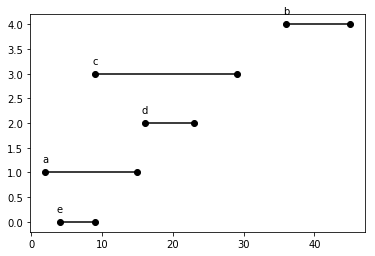
\includegraphics[width=0.48\columnwidth]{fig/greedy_schedule_all_intervals_sorting_finish.png}
        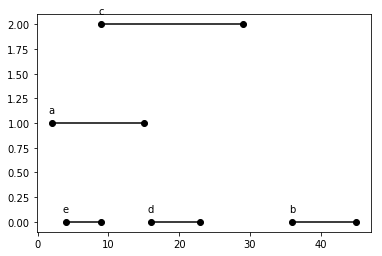
\includegraphics[width=0.48\columnwidth]{fig/greedy_schedule_all_intervals_wrong_sort.png}
    \caption{Left: sort by start time, Right: sort by finish time.}
    \label{fig:greedy_intervals_sorting_bad}
\end{figure}
\begin{figure}[H]
    \centering
    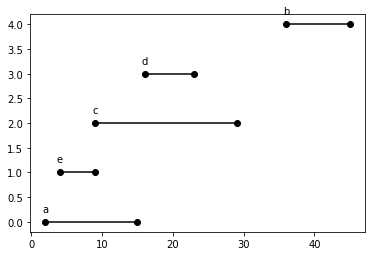
\includegraphics[width=0.48\columnwidth]{fig/greedy_schedule_all_intervals_sorting.png}
        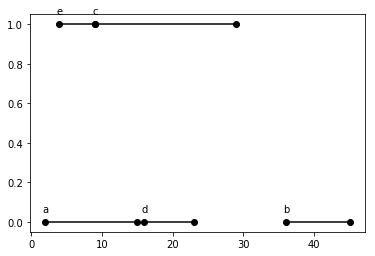
\includegraphics[width=0.48\columnwidth]{fig/greedy_schedule_all_intervals_good_sort.png}
    \caption{Left: sort by start time, Right: sort by finish time.}
    \label{fig:greedy_intervals_sorting_good}
\end{figure}
Unfortunately, it gives us wrong answer; it used three resources instead of 2 as we proved before. The sorting and the answer is plotted in  Fig.~\ref{fig:greedy_intervals_sorting_bad}. What went wrong? In the non-overlapping interval scheduling problem, what matters is the maximum number of intervals we can fit in within one resource, sorting by finish time guarantees we fit as many intervals as possible. However, in this problem, we try to use as less as possible of resources, we want each resource to be as tight as possible. In math, .... Therefore, the right way of sorting is to sort by the starting time. If you insist on sorting by finish time, you will get right answer if you traverse the intervals in reversed order.  

This type of assignment takes $O(n^2)$ in time complexity. We can easily do better but with the same greedy strategy. 
\subsubsection{Optimizations} 
We use a list \texttt{rooms} which starts as being empty.  Each room, we only keep its end time. After sorting by the start time, we go through each interval and try to put it in a room if it does not overlap, we put this interval in this room and update its end time. If no available room found, we assign a new room instead. With this strategy, we end up with $O(nd)$ in time complexity. When $d$ is small enough, it saves more time. 
\begin{lstlisting}[language=Python]
def minMeetingRooms(intervals):
    intervals = sorted(intervals, key=lambda x: x[0])
    rooms = [] # a list that tracks the end time
    for s, e in intervals:
        bFound = False
        for i, re in enumerate(rooms):
            if s >= re:
                rooms[i] = e
                bFound = True
                break
        if not bFound:
            rooms.append(e)
    return len(rooms)
\end{lstlisting}
\paragraph{Priority Queue} Is there a way to fully get rid of the factor of $d$? In our case, we loop over all rooms and check if it is available, but we do not even care which one is, we just need one! So, instead we replace \texttt{rooms} with a priority queue with uses min-heap, making sure each time we only check the room with the earliest end time; if it does not overlap, put this meeting into this room and update its finish time,  or else assign a new room.
\begin{lstlisting}[language=Python]
import heapq
def minMeetingRooms(intervals):
    intervals = sorted(intervals, key=lambda x: x[0])
    rooms = [] # a list that tracks the end time of each room
    
    for s, e in intervals:
        bFound = False
        # now, just check the room that ends earlier instead of check it all
        if rooms and rooms[0] <= s:
            heapq.heappop(rooms)
        heapq.heappush(rooms, e)
    return len(rooms)
\end{lstlisting}
\subsection{Partition} 
\paragraph{763. Partition Labels}   A string S of lowercase letters is given. We want to partition this string into as many parts as possible so that each letter appears in at most one part, and return a list of integers representing the size of these parts.

\begin{lstlisting}[numbers=none]
Example 1:

Input: S = "ababcbacadefegdehijhklij"
Output: [9,7,8]
Explanation:
The partition is "ababcbaca", "defegde", "hijhklij".
This is a partition so that each letter appears in at most one part.
A partition like "ababcbacadefegde", "hijhklij" is incorrect, because it splits S into less parts.
\end{lstlisting}

\begin{lstlisting}[numbers=none]
for example ``abaefegdehi''.
{aba}, {efegde}, {hi}
\end{lstlisting}
\paragraph{Analysis} We know we can use the partition type of dynamic programming to find the maximum length with
\begin{align}
    d[n] = p[i:n],  d[i] \\
    d[n] = \max(d[i] + 1), i < n, \texttt{and p[i:n] is   an independet part}.\\
    d[i] = p[j:i], d[j], i\in[0, n-1], j<i, \\
    d[i] = \max(d[j] + 1)
\end{align}
This will give us a solution with $O(n^2)$. Not bad! In dynamic programming solution, when we are solving subproblem ``abaefegdeh'', we are checking all previous subproblems' solutions. However, if we observe, we only need the optimal solutions of the previous subproblem ``abaefegde''-- ``aba'', ``efegde'' to figure out the optimal solution of current: simply check if 'h' is in any parts of the preceding optimal solution and merging parts between the earliest part that incorporates 'h' to the last.  Now, we  can also observe that between subproblems for example ``abaefegdehi''.
\begin{lstlisting}[numbers=none]
a, o = {a}
ab, o = {a}, {b}
aba, merge, o ={a,b}
abae, o={a, b}, {e}
abaef, o = {a, b}, {e}, {f}
abaefe, e exists, merge, o = {a, b}, {e, f}
abaefeg
abaefegd
abaefegde
abaefegdeh
abaefegdehi
\end{lstlisting}
This indeed is already a greedy algorithm. We no longer just blindly care about the subprobelm state, but we explicitly working on a single partial optimal solution. We incrementally construct  the partial optimal solution till it is optimal globally. Moreover, we can detect it has unnecessary work to track these optimal solutions,  we can utilize a \texttt{dict} structure to track the last location of a character is seen in the string. We loop through the characters in the string one by one, and track a subarray's start and end location in the string. Whenever a new character comes, it can either enlarge this part, or within the last range, or it is the end of the range and different type of process is applied for different case. The Python code shows more details of this greedy approach algorithm:
\begin{lstlisting}[language=Python]
from collections import defaultdict
class Solution:
    def partitionLabels(self, S: str) -> List[int]:
        n = len(S)
        loc = defaultdict(int)
        for i, c in enumerate(S):
            loc[c] = i # get the last location of each char
        last_loc = -1
        prev_loc = -1
        ans = []
        for i, c in enumerate(S):
            #prev_loc = min(prev_loc, i)
            last_loc = max(last_loc, loc[c])
            if i == last_loc: ##a good one                
                ans.append(last_loc - prev_loc)
                prev_loc = last_loc
                
        return ans
\end{lstlisting}
With the greedy approach, we further decreased the complexity to $O(n)$. 
\subsection{Data Compression, File Merge}
\paragraph{File Merge}
Given array $F$ of size $n$, each item indicates the length of the $i$-th file in the array. Find the best ordering of merging all files. 
\begin{lstlisting}[numbers=none]
For example, F = {10,5,100,50,20,15}
\end{lstlisting}
First, this is a exponential problem because we might need to try all permutation of a file. Merge the first two files take 10+5 cost, and merge this further with 100, takes 10+5+100, and so. Now, let us write the cost of the original order:
\begin{align}
    c &= \min (F_0+F_1) + (F_0+F_1+F_2) + ... + (F_0+F_1+F_2+...+F_{n-1}) \\
    &=\min(n-1) F_0 + (n-2) F_1+ ...+F_{n-1}
\end{align}
From the objective function, because all file size are having positive sizes, to minimize it, we have to make sure $F_0$ is the smallest item in the array because it has to be computed the most times, and $F_2$ is the second smallest and so on. We can easily figure out that sorting the files in increasing orders and merge them in this order result the least cost of merging. This is a very simple and natural greedy approach. 
\paragraph{Data Compression}
\subsection{Factional S}
\subsection{Graph Algorithms}
%%%%%%%%%%%%%%%%%%%%%%%%Exercise
\section{Exercises}
\begin{itemize}
    \item 630. Course Schedule III (hard)
\end{itemize}


%We shall complete the process of developing a greedy solution by converting the recursive algorithm to an iterative one. Although the steps we shall go through in this section are slightly more involved than is typical when developing a greedy algorithm, they illustrate the relationship between greedy algorithms and dynamic programming.
\end{document}